%\documentclass[12pt, a4paper]{scrartcl}
%\usepackage[ngerman]{babel}
%\usepackage[utf8]{inputenc}

%\begin{document}
\section{Entwurf und Umsetzung der Netzwerk-Schnittstelle}
\subsection{Grundlegende Theorie zur Kommunikation in einem Netzwerk}
Unter dem Begriff Netzwerk im Zusammenhang mit dieser Arbeit wird, sofern es nicht ausdrücklich anders definiert ist, die Ansammlung mehrerer, untereinander verbundener Computer verstanden.
Diese haben die Möglichkeit mit standardisierten Internet-Netzwerkprotokollen miteinander zu kommunizieren.
Diese Kommunikation wird beschrieben durch das ISO/OSI Modell (s. \glsref{ISO/OSI Modell}) der Netzwerkkommunikation, auf dem auch die Arbeitsweise unseres Programmes aufbaut.
Dabei kann man den Prozess, welcher bei einer Netzwerkübertragung abläuft und die verwendeten Informationen in Schichten nach ihrem Abstraktionsgrad einteilen, von Nullen und Einsen in einem Kabel bis hin zu z.B. verschiedensten Verschlüsselungsprotokollen; was in unteren Schichten abgesichert ist, muss in denen darüber nicht implementiert werden, was wiederum zu einfachen und verlässlichen einzelnen Algorithmen in einer Schicht führt, obwohl das gesamte System überaus komplex ist.

\subsection{Notwendigkeit, Anforderungen und Spezifikation eines eigenen Netzwerkprotokolls}
Um das Programm zu dritt zu entwickeln, muss eine gewisse Modularität gewährleistet werden, außerdem müssen die Sinnabschnitte klar nach ihrer Funktion gegliedert sein und eine leicht benutzbare sowie wiederverwendbare Schnittstellen besitzen, damit nicht das gesamte Programm angepasst werden muss, wenn ein Teil geändert wird und jeder sich auf seinen Teil konzentrieren kann, ohne die anderen vollständig zu kennen.
Diese Anforderungen werden durch die Trennung der Programmiersprachen Lua und C++ einfach geregelt, aber in reinem C++ Kontext muss es dennoch eine Unterteilung zwischen Netzwerkschnittstelle und Benutzeroberfläche geben, weshalb die gesamte Netzwerkkommunikation über eine statische Bibliothek in die ausgeführte Datei eingebunden ist, in dem die Benutzeroberfläche und die Verbindung der Programmteile gemacht werden.
Die Aufgabe der Bibliothek ist, eine verlässliche Verbindung zwischen zwei Rechnern aufzubauen (Start und Ziel), über die ein fester Satz von Anweisungen mit optionalen Argumenten sowie Dateien bidirektional übertragen werden können.
Dafür stellen sich folgende Anforderungen, es muss:

\begin{itemize}
\item ein gesicherter Transport von beliebigen Daten möglich sein,
\item eine verschlüsselte Kommunikation vorliegen
\item der Datenverkehr so klein wie möglich sein
\item der Kommunikationskanal in beide Richtungen gleich aufgebaut sein und
\item die Übertragung auch von größeren Dateien mit zusätzlichen Informationen fehlerfrei ablaufen
\end{itemize}

Diese Bedingungen implizieren bereits, dass eine bestimmte Regelung und einen Ablauf für die Kommunikation zwischen den beiden Computern geben muss: ein Protokoll (s. \glsref{Protokoll}).\par
Alle oben genannten Anforderungen müssen durch dieses Protokoll erfüllt sein und geregelt werden; daher umfasst es sowohl einen bestimmten Datensatz, der in den Header (s. \glsref{Header}) eines Pakets (s. \glsref{Paket}) geschrieben wird als auch einen festgelegten Ablauf der Kommunikation, der sicherstellt, dass alle Daten korrekt angekommen sind und verarbeitet wurden.\par 
Um nicht ebenfalls für die sichere Ankunft der Daten sorgen zu müssen, baut das Protokoll auf TCP/IP auf (genauer auf dem Protokoll TLS, welches auch eine verschlüsselte Verbindung aufbaut), also der Transportschicht des ISO/OSI-Modells, auf der bereits genau das implementiert und standardisiert ist - praktisch ist unser Protokoll also auf der Anwendungsschicht des Modells.
Da das Protokoll sowohl für den Versand von Anweisungen als auch für den von Dateien geeignet sein muss und dabei so wenig Datenverkehr wie möglich verursachen soll (\textit{= leichtgewichtig}), gibt es zwei verschiedene Teilprotokolle, was in folgendem Aufbau der Kommunikationsstruktur resultiert:\par
Im ersten Schritt werden zwei Informationen, als Zahlen codiert, zum Typ der Übertragung, also Anweisung oder Datei, und zu ihrer Gesamtgröße in den Header des ersten Pakets der Übertragung geschrieben.
Abhängig davon, was der Übertragungstyp ist, wird nun entweder die Informationen für eine Dateiübertragung oder eine Anweisungsübertragung angehängt.
Dabei sind alle Werte, sofern es möglich ist, als Zahlen und nicht als Zeichenketten vorhanden, um die Größe der Informationen zu minimieren.\\\par
Betrachtet man zunächst den Header für die Anweisungen, so braucht man einen Anweisungscode, der am Zielort eindeutig zu einer Anweisung zugeordnet werden kann; Teil zwei sind Standardargumente, die binär auf 32 Bit Speicherbreite gespeichert werden.
Dabei soll zum Beispiel, wenn das erste Bit auf eins gesetzt wurde, die Anweisung "`Rufe eine Liste der Daten ab, auf die Das Programm Zugriff hat"' nur die Ordnerstruktur herüberschicken, ist das zweite Bit auf eins gesetzt soll es zusätzliche Informationen zur Größe oder den Zugriffsrechten auf die Dateien mitsenden; dafür wären anderenfalls eigene Anweisungen nötig, was der Übersichtlichkeit bei der Implementierung abträglich wäre und deshalb bereits im Protokoll integriert ist.\par 
Der dritte Wert im Headersegment für die Anweisungen ist eine Zahl, die ein Programm identifiziert, auf dass die Anweisung angewendet werden soll, was standardmäßig das Eigene ist.
Der vierte Wert ist eine Längenangabe in Bytes.
Er bezeichnet die Länge eines optionalen Argumentes, welches an den Header angehängt werden kann, beispielsweise ein Dateiname oder eine Chat-Nachricht.\par 
Um die ganze Anweisung klein zu halten wird intern festgelegt, dass die Gesamtgröße dieses Headersegments inklusive des optionalen Arguments nicht größer als $2^{16}$ Byte sein darf.
Aus Kompatibilitätsgründen mit verschiedenen Compilern und Systemen sind alle Werte Integer mit 32 bzw. 64 Bit Speicherbreite, um damit sowohl genügend Platz für alle Informationen zu bieten als auch Probleme mit verschiedenen Rechnerarchitektur-spezifischen Anpassungen der Speicherbreite zu vermeiden.
Insgesamt ergibt sich also folgende Spezifikation des Headers für die Versendung von Anweisungen (Abb. \ref{Anweisungs_Header}):\par

\begin{figure}[h] 
\begin{lstlisting}
     0                   1                   2                   3
     0 1 2 3 4 5 6 7 8 9 0 1 2 3 4 5 6 7 8 9 0 1 2 3 4 5 6 7 8 9 0 1
    +-+-+-+-+-+-+-+-+-+-+-+-+-+-+-+-+-+-+-+-+-+-+-+-+-+-+-+-+-+-+-+-+
    |                        Anweisungscode                         |
    +-+-+-+-+-+-+-+-+-+-+-+-+-+-+-+-+-+-+-+-+-+-+-+-+-+-+-+-+-+-+-+-+
    |                       Standardargumente                       |
    +-+-+-+-+-+-+-+-+-+-+-+-+-+-+-+-+-+-+-+-+-+-+-+-+-+-+-+-+-+-+-+-+
    |                        Zielprogramm-ID                        |
    +-+-+-+-+-+-+-+-+-+-+-+-+-+-+-+-+-+-+-+-+-+-+-+-+-+-+-+-+-+-+-+-+
    |             Länge des optionalen Arguments in Byte            |
    +-+-+-+-+-+-+-+-+-+-+-+-+-+-+-+-+-+-+-+-+-+-+-+-+-+-+-+-+-+-+-+-+
    |              optionales Argument variabler Länge              |
    +-+-+-+-+-+-+-+-+-+-+-+-+-+-+-+-+-+-+-+-+-+-+-+-+-+-+-+-+-+-+-+-+
\end{lstlisting}
\caption{Header für Anweisungen}
\label{Anweisungs_Header}
\end{figure}

\begin{figure}[h]
\begin{lstlisting}
	0                   1                   2                   3
    0 1 2 3 4 5 6 7 8 9 0 1 2 3 4 5 6 7 8 9 0 1 2 3 4 5 6 7 8 9 0 1
   +-+-+-+-+-+-+-+-+-+-+-+-+-+-+-+-+-+-+-+-+-+-+-+-+-+-+-+-+-+-+-+-+
   |                           Dateiart                            |
   |                                                               |
   +-+-+-+-+-+-+-+-+-+-+-+-+-+-+-+-+-+-+-+-+-+-+-+-+-+-+-+-+-+-+-+-+
   |                 Länge des Dateinamens in Byte                 |
   |                                                               |
   +-+-+-+-+-+-+-+-+-+-+-+-+-+-+-+-+-+-+-+-+-+-+-+-+-+-+-+-+-+-+-+-+
   |                  Länge der Prüfsumme in Byte                  |
   |                                                               |
   +-+-+-+-+-+-+-+-+-+-+-+-+-+-+-+-+-+-+-+-+-+-+-+-+-+-+-+-+-+-+-+-+
\end{lstlisting}
\caption{Header für Dateiübertragungen}
\label{Datei_Header}
\end{figure}

Dabei ist die Länge der Argumente in (pro Zeile 32) Bit angegeben, sofern nicht anders spezifiziert.\\\\
Das Versenden von Dateien hat andere Anforderungen, was in einem anderen Aufbau des Header-Segments für eine solche Übertragung, sowie in einem anderen Ablauf resultiert.\par
Für jede Dateiübertragung wird, im Gegensatz zu den Anweisungen, jeweils eine neue TLS-Verbindung aufgebaut(Schritt 0), die unabhängig von vorhergehenden und nachfolgenden ist, es gibt also für jede Datei einen abgeschotteten "`Kanal"', in dem Fehler leicht behandelbar und konkurrierende Übertragungen unmöglich sind.
Danach wird ein Paket mit Informationen zu der Datei zum Zielcomputer geschickt(Schritt 1), welcher, um die Integrität der Übertragung zu verifizieren, dasselbe Paket zurücksendet(Schritt 2).\\

\begin{wrapfigure}{r}{.65\textwidth}
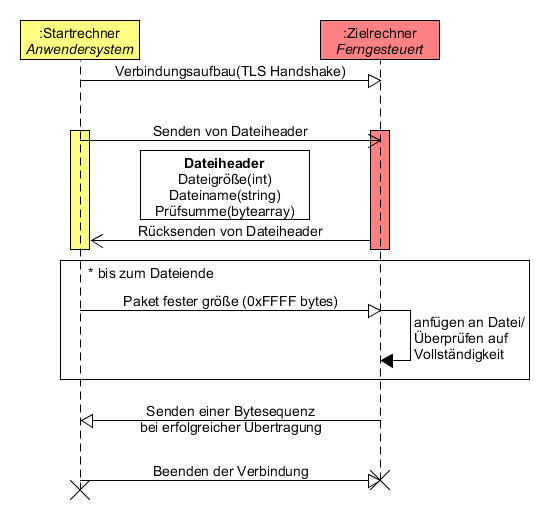
\includegraphics[scale=.4]{diagramFileProtocol}
\caption{Schematische Darstellung des Ablaufs bei der Dateiübertragung}
\label{file_diagram}
\end{wrapfigure}

Dieses Informationspaket ist in Abbildung \ref{Datei_Header} schematisch dargestellt.
Es besteht aus der Art der Datei (z.B. Video, Audio, Text, ausführbare Dateien etc.), was in der weiteren Einordnung im Zielcomputer nützlich ist, dem ursprünglichen Dateinamen und einer Prüfsumme, mit der die fehlerfreie Ankunft verifiziert werden kann.\\
Das Headersegment ist daher so aufgebaut, dass zunächst die drei Ganzzahlwerte für Typ, Länge des Dateinamen in Byte und Länge der Prüfsumme in Byte in den Header geschrieben werden. Dann werden Dateinamenslänge und Prüfsumme angehängt und dieses gesamte Paket wird an den Zielcomputer übermittelt.\par
Ist die Verbindung verifiziert, wird mit der eigentlichen Übertragung der Datei begonnen, die in kleinen Abschnitten und ohne weitere Kennzeichnung in mehreren kleinen Paketen geschieht(Schritt 3 bis x).
Das funktioniert, da unser Standard auf TCP/IP aufbaut, welcher bereits die richtige Reihenfolge und Vollständigkeit der Pakete weitgehend sicherstellt und nur eine Verbindung pro Dateiübertragung aktiv ist.
Am Zielcomputer wird die Datei schließlich in einem temporären Standardverzeichnis abgespeichert und Paket für Paket zusammengesetzt.
Ist die Übertragung nach dem Senden einer bestimmten Bytesequenz vom Zielcomputer beendet, wird ein Signal aus der Managerklasse ausgesendet und die Verbindung getrennt.
Diese Schrittfolge ist schematisch in Abbildung \ref{file_diagram} dargestellt.
Nach dem erfolgreichen Übertragen wird noch mit der anfänglich verschickten Prüfsumme der Datei die Integrität der Datei geprüft, um Fehler insgesamt auszuschließen.

\subsection{Funktionsumfang der selbstgeschriebenen Klassenbibliothek}
Die Bibliothek stellt auf oberster Ebene eine Schnittstelle zum Übertragen von Dateien und Anweisungen zu einer bekannten Adresse, welche in angemessener Form codiert sind.
Das heißt konkret, es werden Methoden bereitgestellt, welche die einzelnen Informationen in das passende Format das einfach verschickt werden kann umwandeln, dargestellt durch zwei Klassen, die die nötigen Informationen, also z.B. Dateiprüfsummen, Dateinamen, Anweisungen usw., so verpacken, dass diese dann einfach vom darunterliegenden System verarbeitet werden können.
Zusätzlich dazu ist natürlich eine entsprechende Fehlerbehandlung bei Verbindungsabbrüchen oder fehlerhaften Übertragungen und die Möglichkeit eine Fortschrittsmeldung bei der Dateiübertragung implementiert.
Insgesamt muss der Programmierer nur mit zwei Klassen interagieren, um die volle Funktionalität der Bibliothek ausnutzen, was das gesamte Konstrukt sehr gut für weitere Verwendungen in flexiblen Kontexten der modularen Programmierung eignet und gute Modularität bietet.

\subsection{Implementierung und Funktionsweise der Klassenbibliothek}

\begin{wrapfigure}{r}{.55\textwidth}
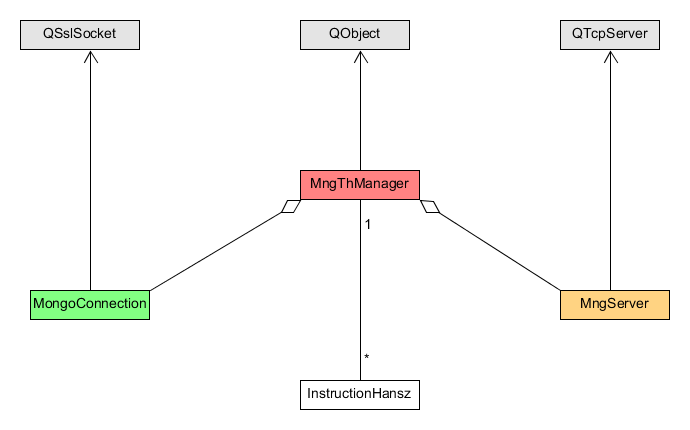
\includegraphics[scale=.4]{classDiagInstr}
\caption{Schematisch: Anweisungsversand}
\label{inst_d}
\end{wrapfigure}

In der Bibliothek sind neben den beiden oben beschriebenen Manager-Klassen (MngThManager für Dateien und MngFileManager für Dateien) mehrere andere Klassen definiert, welche von den jeweiligen Manager-Klassen aus aufgerufen und benutzt werden und dadurch eine darunterliegende Schicht bilden, die durch eine fest definierte Schnittstelle an den Rest des Programms angebunden werden.
Außerdem gibt es eine von allen Klassen benutzte Datei, in denen die Datenstrukturen und Datentypen, die in den Header der Pakete geschrieben werden, als C-Structs definiert sind und einige Funktionen, die häufig gebraucht werden (z.B. String-Vervielfältigung, eine hexadezimale Ausgabe und eine Funktion zum errechnen der Dateiprüfsumme) deklariert; die Definition erfolgt in einer zugehörigen Datei.\par
Der Aufbau der Übertragung beider Datentypen, die verschickt werden, ähnelt sich bis zu einem gewissen Punkt - so haben beide eine eigene Klasse, in der intern die Objekte(Anweisungen und Dateizugriffsobjekte) gespeichert sind und verwaltet werden: (\textit{FileHansz} bzw. \textit{InstructionHansz}), sowie andere Klassen zum Verbindungsaufbau und dem Versand: Eine Klasse, die für das Annehmen von hereinkommenden Verbindungen zuständig ist und eine(bei Dateien zwei) Socket-Klassen, die sich um das Senden bzw. Empfangen von Daten kümmern, was in Abb. \ref{inst_d} bzw. \ref{file_d} vereinfacht schematisch dargestellt ist.\\\\
Die beiden Speicherklassen werden dabei sowohl für den Empfang als auch das Senden eines Objektes genutzt - im ersten Fall werden sie mit den Teildaten(also Anweisungscode und zusätzlichen Argumenten oder Dateiname und Dateityp)
 initialisiert und erstellen daraus einen Pufferspeicher, der bereits den korrekten Header und das Datenpaket enthält, dessen Inhalt dann nur noch ausgelesen und verschickt werden muss - somit ist ein gleicher Aufbau der Verbindung in beide Richtungen sichergestellt.\par
Das tatsächliche Versenden, sowie der Verbindungsaufbau wird von einer "`Server"'-Klasse und den Socket-Klassen übernommen.
Dabei horcht die Serverklasse, sowohl für Dateien als auch für Anweisungen auf der Empfangenden Seite auf einem zuvor bestimmten Port auf eingehende Verbindungen.
Auf der sendenden Seite wird eine neue Klasse erstellt, welche ein TLS-Socket initialisiert und zu der gegebenen Adresse verbindet.
Ist die Verbindungsanfrage eingegangen, wird eine normale TLS-gesicherte Verbindung aufgebaut, sofern das möglich ist; danach weichen die Abläufe von Dateiversand und Anweisungsübertragung ab: Anweisungen werden jetzt, in der Reihenfolge in der sie eingehen, von der Managerklasse an das Socket getaktet weitergeleitet, wo sie dann inklusive Header und Datenpaket verschickt werden - bei Dateien ist der Ablauf etwas komplexer.\par

\begin{wrapfigure}{r}{.55\textwidth}
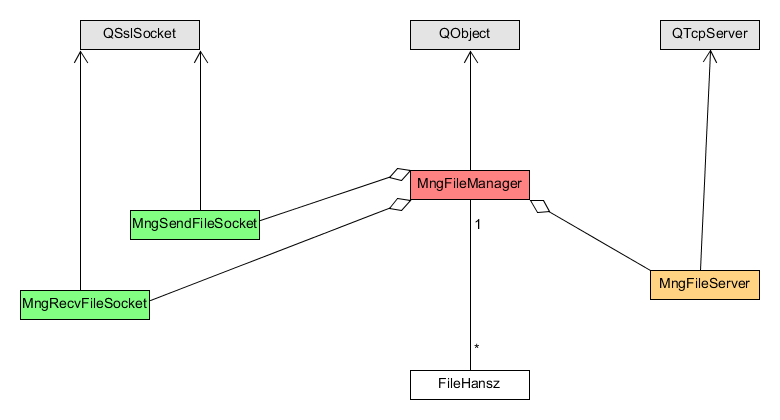
\includegraphics[scale=.35]{classDiagFile}
\caption{Schematisch: Dateiversand}
\label{file_d}
\end{wrapfigure}

Dabei muss zunächst erwähnt werden, dass für Dateien, im Gegensatz zu Anweisungen jedes Mal eine neue Verbindung aufgebaut wird.
In der Verbindung für eine Datei wird, sobald sie aufgebaut ist, zuerst der Header für die Dateiübertragung an den Zielcomputer gesendet(1), welcher genau dasselbe Paket dann zurückschickt(2) um sicherzustellen, dass alle Steuerinformationen korrekt angekommen sind.
Jetzt wird die eigentliche Übertragung der Datei gestartet, welche mit dem Auslesen eines Datenblockes fester Größe beginnt(3).
Dieser wird in einen Pufferspeicher geschrieben, der, wenn er voll ist von der Socket-Klasse ausgelesen und übertragen wird(4); diese Anweisungsfolge(3 und 4) wird so lange wiederholt, bis das Ende der Datei erreicht ist.
Der letzte Datenblock enthält oft weniger als die Maximalgröße, was aber in der Praxis kein Problem ist - das letzte Datenpaket auf der Seite des verschickenden Rechners ist nur etwas kleiner als der Rest.
Auf der empfangenden Seite werden die ankommenden Datenpakete über ihre Repräsentation als FileHansz-Objekt in eine nach der Datei-Prüfsumme benannten Datei im Dateisystem gespeichert - das verhindert die konkurrierende Benennung von ungleichen Dateien und vereinfacht das Überprüfen auf korrekte Übertragung; die ursprünglichen Namen werden zu Beginn der Übertragung per Signal an das Programm außerhalb der Bibliothek geschickt, welches diese dann weitergehend speichert.
Sind alle Pakete versandt worden und angekommen, wofür die TCP-basierte Verbindung sorgt, wird vom Empfangenden Rechner eine Bytesequenz übertragen, welche die Erfolgreiche Übertragung kennzeichnet.\par
Danach wird die Verbindung abgeschlossen und die beiden Sockets gelöscht.\\
%\end{document}